\documentclass[letterpaper, 11pt]{article}

\usepackage{lastpage, siunitx, hyperref, amsmath, color, graphicx}

%\definecolor{orange}{rgb}{1,0.5,0}

\def\UrlBreaks{\do\/\do-}

%\usepackage[hyphens]{url}

\usepackage[margin=1in]{geometry}
%\geometry{hscale=.6, vscale=.8, hmarginratio=2:1, vmarginratio=1:1, marginparwidth=.18\paperwidth, ignoremp}
%\geometry{marginparwidth=.1\paperwidth}

%\usepackage[T1]{fontenc}

%\usepackage[explicit]{titlesec}
%\titlespacing*{\section}{\dimexpr -\marginparsep-\marginparwidth}{*4}{*1}
%\titleformat{\section}[runin]{\large\bfseries\titlerule[.5pt]\filright}{\makebox[1em][c]{\thesection}}{1em}{\parbox[t]{\dimexpr\marginparwidth-2em}{#1}\hskip\marginparsep\mbox{}}[\newline\vspace{-4ex}]

%\titlespacing*{\subsection}{\dimexpr -\marginparsep-\marginparwidth}{*4}{*1}
%\titleformat{\subsection}[runin]{\large\bfseries\titlerule[.5pt]\filright}{\makebox[1em][c]{\thesection}}{1em}{\parbox[t]{\dimexpr\marginparwidth-2em}{#1}\hskip\marginparsep\mbox{}}[\newline]

\usepackage{enumitem}
\newlist{steps}{enumerate}{1}
\setlist[steps]{label=Step \arabic*, font=\bfseries, leftmargin=-\marginparsep, itemindent=\marginparsep, align=right}

\usepackage{fancyhdr}
\pagestyle{fancy}
\fancyhf{}
%\fancyhfoffset[lh,lf]{\dimexpr\marginparwidth+\marginparsep}
\fancyhf[lh]{UCD EEC 134}
\fancyhf[ch]{}
\fancyhf[rh]{}
%\fancyhf[lf]{left foot}
%\fancyhf[cf]{centre foot}
\fancyhf[rf]{Page \thepage /\pageref{LastPage}}
%\renewcommand{\footrulewidth}{.4pt}

%%%%%%%%%%%%%%%
%%%% Tikz definitions
%%%%%%%%%%%%%%%
%\tikzstyle{Uno}=[rectangle,fill=white,draw,line width=0.5mm]

%new commands
%display due date in red and link to the eec134-schedule.pdf document
\newcommand{\due}[1]{\href{https://github.com/ucdart/UCD-EEC134/blob/master/support/schedule/eec134-schedule.pdf}{\textcolor{red}{#1}}}

\graphicspath{{./figures/}}

\begin{document}

\title{EEC 134 Quarter 2 Project Guidelines}
\author{Instructor: Xiaoguang ``Leo'' Liu\\lxgliu@ucdavis.edu \\
	\small \href{http://creativecommons.org/licenses/by-sa/4.0/}{CC BY-SA 4.0}}
%\date{}
\date{Last updated: \today}

\maketitle

In Quarter 2 of the EEC 134 course, our main goal is to improve and innovate upon the Quarter~1 radar system. You should strive to build longer range, higher resolution, smaller size, and lower power consumption radar systems.

\section{Quarter 2 Project Technical Requirements}
%There are two project options that you can pursue.

The following section outline the \textit{technical requirements} so that performance of each team can be judged fairly. The grading details of both options will be announced after all teams have registered their choices. A total budget of \textbf{\$300} is allowed for each team. 

%\subsection{Option 1: Radar Performance Competition}
	
%In this option, you will use your radar to measure the distance to various targets. 

Shown in Fig.~\ref{fig:range-competition}, a group of targets will be set up at various distances and bearing angles in an open field. The targets will be 0.3$\times$0.3\,m$^2$ metal plates mounted on wood stands. The maximum and minimum range of the targets are 50 meters and 5 meters, respectively. 

	\begin{figure}[h]
		\centering
		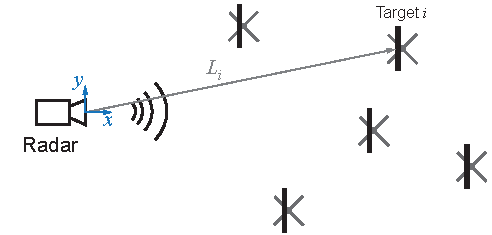
\includegraphics{range-competition}
		\caption{Range competition setup}
		\label{fig:range-competition}
	\end{figure}

Your performance is judged based on a score calculated as follows:
\[
\text{Score} = \frac{P_{dc} \times W}{N} \times \sum_1^N \left( \frac{ \left| \hat{L_i} - L_i \right|}{L_i} \right),
\]
where $P_{dc}$ is the total power consumption of your radar, $W$ is the total weight of your radar, $\hat{L_i}$ is the measured distance to the $i$th target, $L_i$ is the actual distance to the $i$th target, and $N$ is the total number of targets. $N$ will be in the range of 3--5. If you fail to produce a reading for a target, $\hat{L_i}$ will be set to 0, i.e.~$\left| \hat{L_i} - L_i \right|/L_i$ will be 1. Obviously, a smaller score means better performance. 

The only dc power source is a power supply with a single adjustable dc voltage output up to 15\,V. No batteries are allowed on the radar unit. Energy harvesting from ambient sources, e.g.~solar panel, is not allowed. The total weight $W$ of the radar includes the antenna, the RF frontend, and any cable that is used to transfer power or baseband signal.
	
A laptop, smart phone, or tablet can be used for real-time signal processing. The weight of this unit is not counted. If you choose to use an \textbf{on-board signal processor} whose weight will be counted, a bonus multiplier of \textbf{0.2} will be applied to your total score. 

Each team has 15 minutes for taking measurement, processing data, and reporting the result. 

%\subsection{Option 2: Radar Sensor for Unmanned Aerial Vehicles (UAVs)}
%
%The study of agriculture, forestry, hydrology, geology, meteorology, and ecology benefits significantly from spatially explicit remote sensing data to relate structure to function. To date, heavy reliance has been placed on obtaining such data from remote-sensing instruments mounted on spacecraft or manned aircraft, although the spatial and temporal resolutions of the data are often not suited to local-scale ecological investigations. Recent technological innovations have led to an upsurge in the availability of unmanned aerial vehicles (UAVs). Flying low and slow, UAVs offer new opportunities for scale-appropriate measurements. Equipped with capable sensors, UAVs can deliver fine spatial resolution data at temporal resolutions defined by the end user. 
%
%Before small UAVs can be used for autonomous remote sensing, however, critical capabilities in situation awareness, precision location, and multi-modality sensing need to be developed. Small radar sensors are potentially useful for all of the above functionalities. In this project option, your team will be responsible for developing a small radar sensor that satisfies the following requirements. 
%
%\begin{enumerate}[itemsep=-0.1ex]
%	
%	\item The radar sensor needs to have at least 20\,meters of range for a target with RCS of 1\,m$^2$ (show calculation). 
%	
%	\item The radar sensor is to be mounted on a Tarot T-2D 2-axis gimbal for stabilization. The T-2D gimbal is designed to hold a GoPro camera so your radar sensor must fit in the form factor (41\,mm $\times$ 59\,mm $\times$ 30\,mm) and weight (152\,g) of a GoPro camera. 
%	
%	\item The radar sensor needs to include an on-board processor to process and send intensity vs range data back to the UAV flight controller with greater than 10\,Hz refresh rate. Your team has the freedom to define the data transmission protocol. It is OK to use or modify an existing link/protocol, e.g.~serial link. 
%	
%	\item You also need to develop the receiving end of the communication link, e.g.~a computer program running on a computer, to demonstrate that you have a working system. Keep in mind that the UAV will most likely use a single-board computer (SBC), such as the BeagleBone Black or the Intel Edison, that runs a Linux operating system. Although \textbf{not} a requirement for this project option, you may take the computation requirement and program/library availability on the SBC into account when designing your data link/protocol. For example, it may not be realistic to run a full Matlab program on an SBC. 
%	
%	\item The radar sensor needs to work from a 12\,V 1\,A power supply. Any voltage/power conversion should be implemented as part of the sensor system. 
%\end{enumerate}
%
%Grading criteria will be decided upon by the first week of the Winter quarter. Participating teams may propose the grading criteria also. 

\section{Additional Rules}
	\begin{enumerate}[itemsep=-0.1ex]
		
		\item The radar may use any technology as long as it is commercially available. You may choose to design your radar using existing ICs or from individual transistors. Use of commercial microwave/RF subsystems is allowed.
		
		\item The radar shall allow for internal inspection of the circuitry.
		
		\item The radar should not use any external signal source, such as local-oscillator signals or reference clock signals. Using the GPS signal as a reference is allowed but the GPS clock recovery circuit must be included on in the radar system.
		
		\item The radar must operate at room temperature. 		
	\end{enumerate}

\section{Some Tips}
\begin{enumerate}
	\item Sample/purchase 2 or 3 of each component to account for possible assembly errors or the need to have design iterations. 
\end{enumerate}

\section{Quarter 2 Proposal Guidelines}

All teams are required to submit a written proposal describing their quarter 2 project plan by end of day \due{Jan.~25th, 2019}. The proposal needs to address the following aspects.

\begin{enumerate}[itemsep=-0.1ex]
%	\item The project option your team has chosen. 
	
	\item A description of the design of the system including:
		\begin{enumerate}[itemsep=-0.1ex]
			\item A system block diagram showing the major circuit components used in the system.
			
			\item A list of the expected system performance, such as size, weight, power consumption, range, resolution etc. 
			
			\item A calculation of the power/link budget, nonlinearity, and noise figure showing that the system can meet the above specs. 
			
		\end{enumerate}
	
	\item A projected budget based on the above design. The budget should be based on realistic prices of the components used in the systems. Note that the class will offer two free PCB fabrication runs in week 4 and 7. 
	
	\item A timeline showing the proposed system can be built by the end of the Winter quarter. Major milestones, i.e.~what you plan to achieve by when. For example, if part of your project calls for an implementation of the RF circuit using surface-mount components on a PCB, you need to include checkpoints such as when you plan to finish the component selection, component purchase, PCB design, fabrication, and assembly. If possible, include a Gantt chart. 
	 
	\item A clear description of what the role of each group member is. Make sure that each member works on a serious enough portion of the project. 
\end{enumerate} 

\end{document}